\chapter{مدل‌های عصبی}
\section{مقدمه}
از سال ۱۹۵۰ که روزنبلات\footnote{\lr{Rosenblatt}} تئوری پرسپترون\footnote{\lr{Perceptron}}  را ارائه داد\cite{rosenblatt1958perceptron}، مدل‌های شبکه عصبی مصنوعی مختلفی برای شبیه‌سازی ساز و کار زیستی شبکه‌های عصبی ارائه شده است. با این حال اغلب مدل‌ها بر پایه‌ی نورون‌های آنالوگ و اتصالات سیناپسی ساده‌سازی شده با اوزان قابل تنظیم هستند؛ بدون در نظر گرفتن این مهم که مبنای عملکرد نورون، ضربه بوده و سیناپس‌ها دینامیک پیچیده‌ای دارند. در حال حاضر اکثر مدل‌های ارائه شده از تفسیر زیستی مبرا و منحرف شده و بیشتر به سمت تعالی توانایی محاسباتی گرایش دارند. شبکه‌های عصبی ضربه‌ای\footnote{\lr{Spiking Neural Networks}} (SNNs) به عنوان مدل‌هایی که از نظر زیستی انطباق بیشتری دارند، به علت دشواری‌های ذاتی مدل‌سازی آنها، به اندازه‌ی شبکه‌های نورونی آنالوگ در مهندسی محبوب نیستند؛ هرچند که همگان بر این نکته اتفاق نظر دارند که \lr{SNN}ها از نظر محاسباتی توانمند‌تر بوده و به عنوان نسل جدید و انقلابی شبکه‌های عصبی معرفی می‌شوند\cite{ghosh2009spiking}.

گرایش فزاینده‌ای به شبکه‌های عصبی ضربه‌ای، به جهت واقع‌گرایی بیشتر در این گروه از مدل‌ها، در سال‌های اخیر بوجود آمده است. در مدل‌های ضربه‌ای که به عنوان نسل سوم شبکه‌های عصبی معرفی می‌شوند، علاوه بر حالت‌های نورونی و سیناپسی، مفهوم زمان نیز به کار گرفته شده است. نورون‌های SNN دیگر در هر گام آتش نمی‌کنند؛ برخلاف آنچه در شبکه‌هایی مانند پرسپترون چندلایه\footnote{\lr{Multi Layer Perceptron}} داشتیم، بلکه مشابه نورون واقعی زمانی آتش می‌کنند که پتانسیل غشایی آن به یک مقدار مشخص (حد آستانه) برسد. 

\section{شبکه‌های عصبی ضربه‌ای}
\subsection{تاریخچه مدل‌سازی نورونی}
به طور کلی در تاریخچه شبیه‌سازی نورون، سه نسل از شبکه‌های عصبی معرفی شده‌اند که هر کدام بر مبنای مدل‌هایی از نورون هستند که جنبه‌ی خاصی از نورون‌ها را به فرآیند شبیه‌سازی اضافه کرده‌اند. اولین تلاش‌های منجر به شبکه‌های عصبی به سال ۱۹۴۳ میلادی برمی‌گردد؛ زمانی که مک‌کلاچ\footnote{\lr{Warren McCulloch}} و پیتز\footnote{\lr{Walter Pitts}} اولین مدل نورون را ارائه کردند. در مدل آنها یک نورون دارای دو ورودی و یک خروجی بود و فعالیت نورون شبیه‌سازی شده را مشروط به گرفتن ورودی از هر دو شاخه‌ی ورودی کردند. آنها جریان ورودی و خروجی نورون را به شکل دودویی فرض کردند و به همین جهت مدل آنها به «مدار منطق\footnote{\lr{Logic circuit}}» معروف شد. بعدها در دهه‌ی ۵۰ میلادی، محققین در صدد استفاده از این رویکرد جدید برای طراحی شبکه‌های عصبی بهتر برآمدند. روزنبلات\footnote{\lr{Frank Rosenblatt}} یکی از محققین پیشگام در این حوزه بود که در طی تحقیقات خود در مورد بینایی مگس‌ها، در سال ۱۹۵۸، پایه‌ی مدل پرسپترون را بنا کرد. پرسپترون و مدلهای دیگر طراحی شده در آن زمان منجر به یکسری موفقیت‌های ابتدایی شد که متاسفانه به دلیل نگاه غیرواقع‌بینانه و بزرگنمایی‌های رسانه‌ای، با برآورده نشدن یکسری توقعات، باعث دلسردی و در نهایت دوره‌ای رکود در این حوزه شد که به عنوان «زمستان هوش مصنوعی» از آن یاد می‌شود. یکی از دلایل این وقفه که بیش از یک دهه به طول انجامید، کتاب «پرسپترون‌ها» از مینسکی\footnote{\lr{Marvin Minsky}} و پاپرت\footnote{\lr{Seymour Papert}} بود که با بررسی خود، پندار محدودیت‌های غیرقابل غلبه‌ی شبکه‌های پرسپترون که روزنبلات سعی بر زنده نگه داشتن آن داشت بین عموم رواج داد. با وجود آنکه کارهای مهمی مانند ارائه قاعده‌ی پس‌انتشار توسط وربوس همچنان انجام شد، اما سرمایه‌گذاری و حمایت‌های مالی در این دوره بسیار محدود گردید. در اواسط دهه‌ی ۸۰، این زمستان در نهایت به سر آمد و کارهای هاپفیلد\footnote{\lr{John Hopfield}} و روملهارت\footnote{\lr{David Rumelhart}} شوق وسیعی را به تحقیقات شبکه‌های عصبی برگرداند. روملهارت با کشف مجدد روش پس‌انتشار نقش مهمی در احیای شبکه‌های عصبی داشت اما اشتیاق عمومی زمانی مجددا به این سمت روانه شد که هاپفیلد مقاله‌ای در رابطه با شبکه‌های عصبی در آکادمی علوم ملی نوشت اما دیگاه هاپفیلد صرفا محدود به مدل‌سازی نبوده و در پی تکنولوژی‌های کاربردی که به حل مسائل دنیای واقعی منجر شود بود. توجه مجدد به شبکه‌های عصبی و تعداد فزاینده‌ی کنفرانس‌ها و مجامعی که حول این حوزه تشکیل می‌شوند توفیقات فراوانی را به همراه داشته و امروزه شاهد کاربرد‌های وسیع شبکه‌های عصبی، از تشخیص گفتار و چهره تا درمان‌های پزشکی هستیم.

گرچه شبکه‌های پرسپترون با کمک قاعده‌ی پس‌انتشار توفیقات زیادی را کسب کرده‌اند، اما باید این را در نظر داشته باشیم که سطح مدل‌سازی آنها، با آنچه به صورت زیستی در مغز اتفاق می‌افتد بسیار متفاوت است. قانون یادگیری پس‌انتشار پشتوانه‌ی زیستی نداشته و با نظریه‌ی هب که مطرح شد قرابتی ندارد. البته تلاش‌هایی در بکار بردن قانون هب برای شبکه‌های پرسپترون صورت گرفته، اما ساده‌سازی بیش حد نورون‌ها آنها را از حوزه‌ی زیستی بسیار دور کرده است. اعدادی که به عنوان ورودی و خروجی در پرسپترون در نظر گرفته می‌شود نمایانگر نرخ فعالیت (یا تعداد ضربه در یک بازه‌ی زمانی) است در حالی که فعالیت نورون‌ها از یک دینامیک خاص تبعیت کرده و با محدود کردن آن به نرخ فعالیت، ظرفیت محاسباتی پرسپترون بسیار پایینتر از نورون‌های واقعی و مدل‌های ضربه‌ای است. 

\subsection{مدل‌های نورونی}
همانطور که اشاره شد، مدل‌های ضربه‌ای نورون، تلاش دارند تا تفسیر دینامیک وضعیت داخلی نورون که پتانسیل آن را بر اساس ورودی‌های دریافت شده طی زمان تعیین می‌کند به نحوی ارائه دهند که سازوکار نورون واقعی را با سطح مشخصی از جزئیات مدل کند. دینامیک نورون در یک مدل با یکسری معادلات دیفرانسیل مشابه زیر تعیین می‌گردد:

\begin{equation} \label{eq:spiking}
\frac{\partial V}{\partial t} = F(V, I, C)
\end{equation}
که $V$ برداری از متغیرهای مفروض مدل، $I$ جریان ورودی به نورون در هر لحظه و $C$ مجموعه‌ای از پارامترهای تنظیم شده‌ی مدل است. $F$ تابعی است که دینامیک نورون و تغییرات متغیرها بر اساس ورودی و بر حسب زمان را مشخص می‌کند. تابع $F$ ورودی‌های خود را به فضای $\mathbb{R}^n$ می‌برد که $n$ بعد بردار $V$ می‌باشد. به عبارتی دیگر، مدل ضربه‌ای از یک دستگاه معادلات دیفرانسیل از $n$ معادله و $n$ به اضافه‌ی قیدی که با برآورده شدن آن، نورون یک ضربه تولید می‌کند متغیر تشکیل شده است.

مدل‌های نورونی فراوانی ارائه شده‌اند که بسته به پیچیدگی محاسباتی و تطابق زیستی رده‌بندی می‌شوند. ما در این تحقیق از مدل تجمیع و آتش\footnote{\lr{Integrate \& Fire}} (\lr{IF}) و تجمیع و آتش نشتی\footnote{\lr{Leaky Integrate \& Fire}} (\lr{LIF}) استفاده کرده‌ایم که در فصل چهارم با جزئیات بیشتری آنها را تبیین خواهیم کرد. 

\subsection{یادگیری وابسته به زمان ضربه}
نورون‌ها با تغییر در قدرت اتصالات سیناپسی در پاسخ به فعالیت ضربه‌ها، توانایی یادگیری و تطبیق پردازش خود بر حسب تجربه را دارند. 
\lr{STDP} یک نمونه‌ی غیرمتقارن زمانی از قاعده‌ی یادگیری یادگیری هب است که بر اساس همبستگی ضربه‌های نورون‌های پیش و پس‌سیناپسی عمل می‌کند. \lr{STDP} به عنوان مدلی برای شکل‌پذیری سیناپسی در مغز ارائه شده است که بر اساس ترتیب و زمان ضربه‌های پیش و پس‌سیناپسی عمل می‌کند. طبق \lr{STDP}، ضربه‌های پیش‌سیناپسی اگر به طور مکرر چند میلی‌ثانیه پیش از پتانسیل عمل پس‌سیناپسی ظاهر شوند باعث تقویت بلند مدت (LTP) می‌شوند، در حالی که ظهور مکرر ضربه‌ی پس‌سیناپسی قبل از وقوع ضربه‌ی پیش‌سیناپسی به تضعیف بلند مدت (LTD) می‌انجامد. شکل \ref{fig:stdp} تاثیر فاصله‌ی زمانی بین ضربه‌ها بر قدرت سیناپس را که از مشاهدات تجربی \cite{bi1998synaptic} بدست آمده است نمایش می‌دهد. 

\begin{figure}
\centering
{\footnotesize
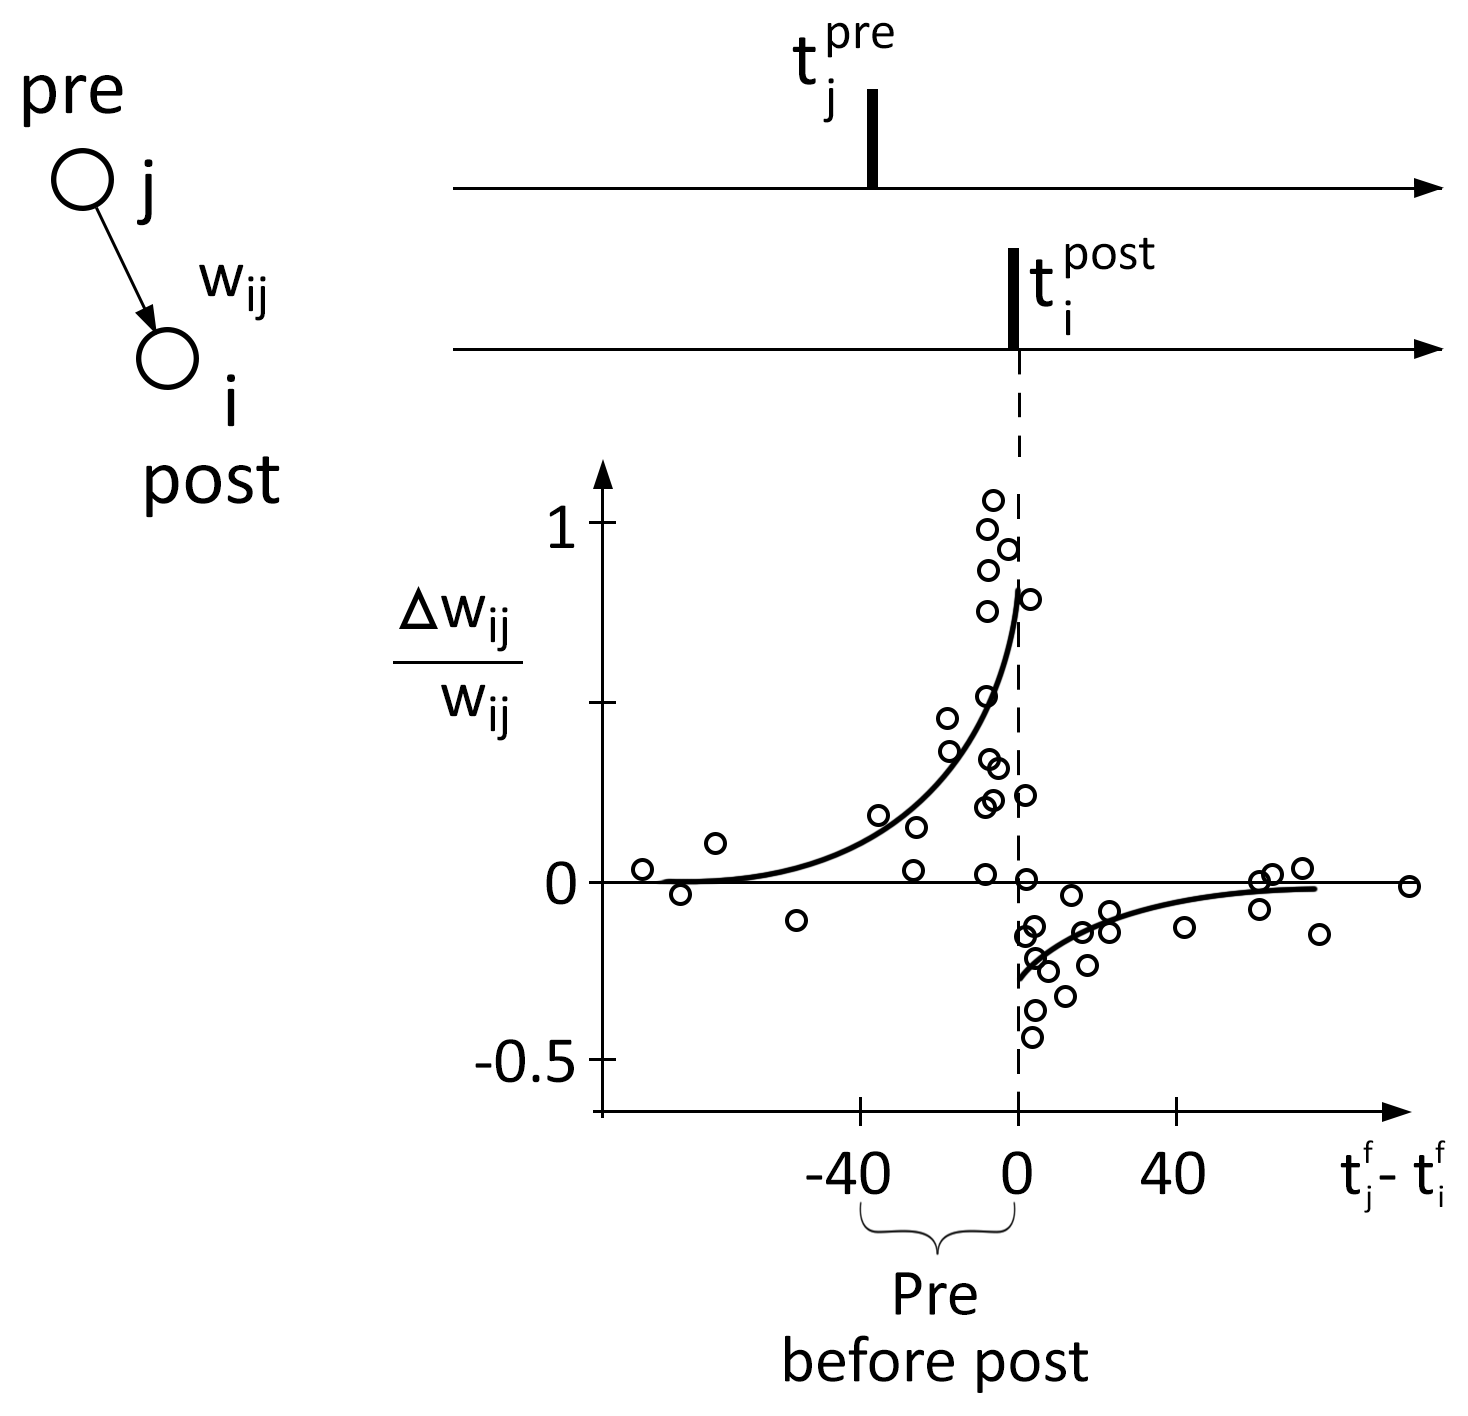
\includegraphics[height=8cm]{stdp}
\caption[یادگیری وابسته به زمان ضربه]{\lr{STDP} تغییرات اتصالات سیناپسی را به صورت تابعی از زمان نسبی بین زوج ضربه‌های پیش و پس‌سیناپسی بیان می‌کند. (ترسیم مجدد از \cite{bi1998synaptic})}
\label{fig:stdp}
}
\end{figure}
معروف‌ترین تابع که برای توجیه این داده‌ها استفاده می‌شود، تابع نمایی است. اگر بخواهیم تغییر وزن سیناپس $j$ را محاسبه کنیم و $t_j^f$ را زمان‌های ضربه‌های نورون پیش‌سیناپسی بگیریم و همچنین زمان آتش‌های نورون پس‌سیناپسی با $t^n$ نمایش داده شود، آنگاه تغییرات وزنی برابر است با:
\begin{equation} \label{eq:stdp1}
\Delta w_j = \sum_f\sum_nW(t^n-t^f_j)
\end{equation}
که $W(s)$ همان تابع \lr{STDP} است که تغییرات وزنی بر مبنای تفاضل زمان ضربه‌ها را تفسیر می‌کند. یک انتخاب محبوب برای این تابع به صورت زیر می‌باشد:

\begin{equation} \label{eq:stdp2}
W(s) =  \left\{\begin{matrix}
A_+exp(-\frac{s}{\tau_+}) & if \;s\geqslant 0\\ 
-A_-exp(-\frac{s}{\tau_-}) & if \; s<0
\end{matrix}\right.
\end{equation}
که برای برازش داده‌های تجربی \cite{zhang1998critical} و مدل‌سازی \cite{song2000competitive} به دفعات استفاده شده است. 
ضریب‌های $A_+$ و $-A_-$ ممکن است به مقدار وزن فعلی $w_j$ وابسته باشند. ثابت‌های زمانی $\tau_-$ و $\tau _+$ نیز در حدود چند ده میلی‌ثانیه انتخاب می‌شوند. تابع \lr{STDP} استفاده شده در این تحقیق در فصل چهار بیان خواهد شد.


\section{یادگیری بدون نظارت ویژگی‌های بصری توسط \lr{STDP}}
قیدهای زمانی که برای مدل‌های بازشناسی الگو در قشر گذاشته می‌شود یکی از چالش‌های اصلی این حوزه است. ثبت‌های صورت گرفته از قشر \lr{IT} میمون نشان داده که تنها در حدود ۱۰۰ میلی‌ثانیه بعد از آغاز محرک، اطلاعات ارزشمند و دقیقی از ماهیت محرک بینایی پردازش می‌شود\cite{hung2005fast}. به احتمال زیاد این نوع پردازش سریع بر توانایی دستگاه بینایی در یادگیری بازشناسی اشکال بصری آشنا، به یادگیری بدون نظارت متکی است. اینکه چگونه این یادگیری صورت می‌پذیرد از چالش‌های اصلی علوم اعصاب نظری می‌باشد. 
مدل بررسی شده در اینجا در سال ۲۰۰۷ توسط ماسکولیه و تورپ\cite{masquelier2007unsupervised} ارائه شده است و دو ویژگی اصلی دارد: اول اینکه با نمایش آنی\footnote{\lr{Flash}} محرک بینایی، نورون‌های موجود  در لایه‌های مختلف به صورت غیرهمزمان آتش می‌کنند به این صورت که نورون‌هایی که قوی‌تر فعال شده‌اند زودتر آتش می‌کنند. نشان داده شده است که این مکانیسم به صورت بهینه اطلاعات تصویر را کد می‌کند\cite{Rullen_2001}.  دوم آنکه نورون‌های مراحل موخر، شکل‌پذیری وابسته به زمان ضربه (\lr{STDP}) را پیاده می‌کنند که می‌دانیم در اثر آن وزن‌های بالای سیناپسی روی سیناپس‌های آوران\lr{Afferent} که به طور قاعده‌مند زود آتش می‌کنند متمرکز می‌شود\cite{guyonneau2005neurons,song2000competitive}. 

با تکرار نمایش تصاویر به این شبکه‌ی پیش‌خور پیچشی و سلسله مراتبی\footnote{\lr{Hierarchical convolutional network}}، مشاهده می‌شود که نورون‌های سطوح میانی به الگوهایی که به طور قابل اطمینان ورودی را عرضه می‌کنند گزیننده\footnote{\lr{Selective}} می‌شوند و تاخیرشان کاهش می‌یابد که در نتیجه باعث پاسخ‌های سریع کارآمد می‌شود. این فرآیند کاملا بدون نظارت صورت می‌گیرد و این ویژگی‌ها را می‌توان برای دسته‌بندی محرک‌ها استفاده کرد.

این مدل، ساختار پیشنهادی سِره، وُلف و پوژیو\cite{serre2005object} که خود مدل \lr{HMAX} را بسط می‌دهد الگوبرداری کرده است و در تلاش برای نمایش پیچیدگی و ناوردایی\footnote{\lr{Invariance}} فزاینده در طور مسیر شکمی، ساختاری چهار لایه (\lr{S1}-\lr{C1}-\lr{S2}-\lr{C2}) را تشکیل می‌دهد که در آن سلول‌های ساده (S) گزینندگی‌شان را از یک عملیات جمع خطی بدست می‌آورند در حالی که سلول‌های پیچیده (C) ناوردایی را با یک عملیات ادغام بیشینه\footnote{\lr{Max pooling} } خطی فراهم می‌کنند. 

\begin{figure}
\centering
{\footnotesize
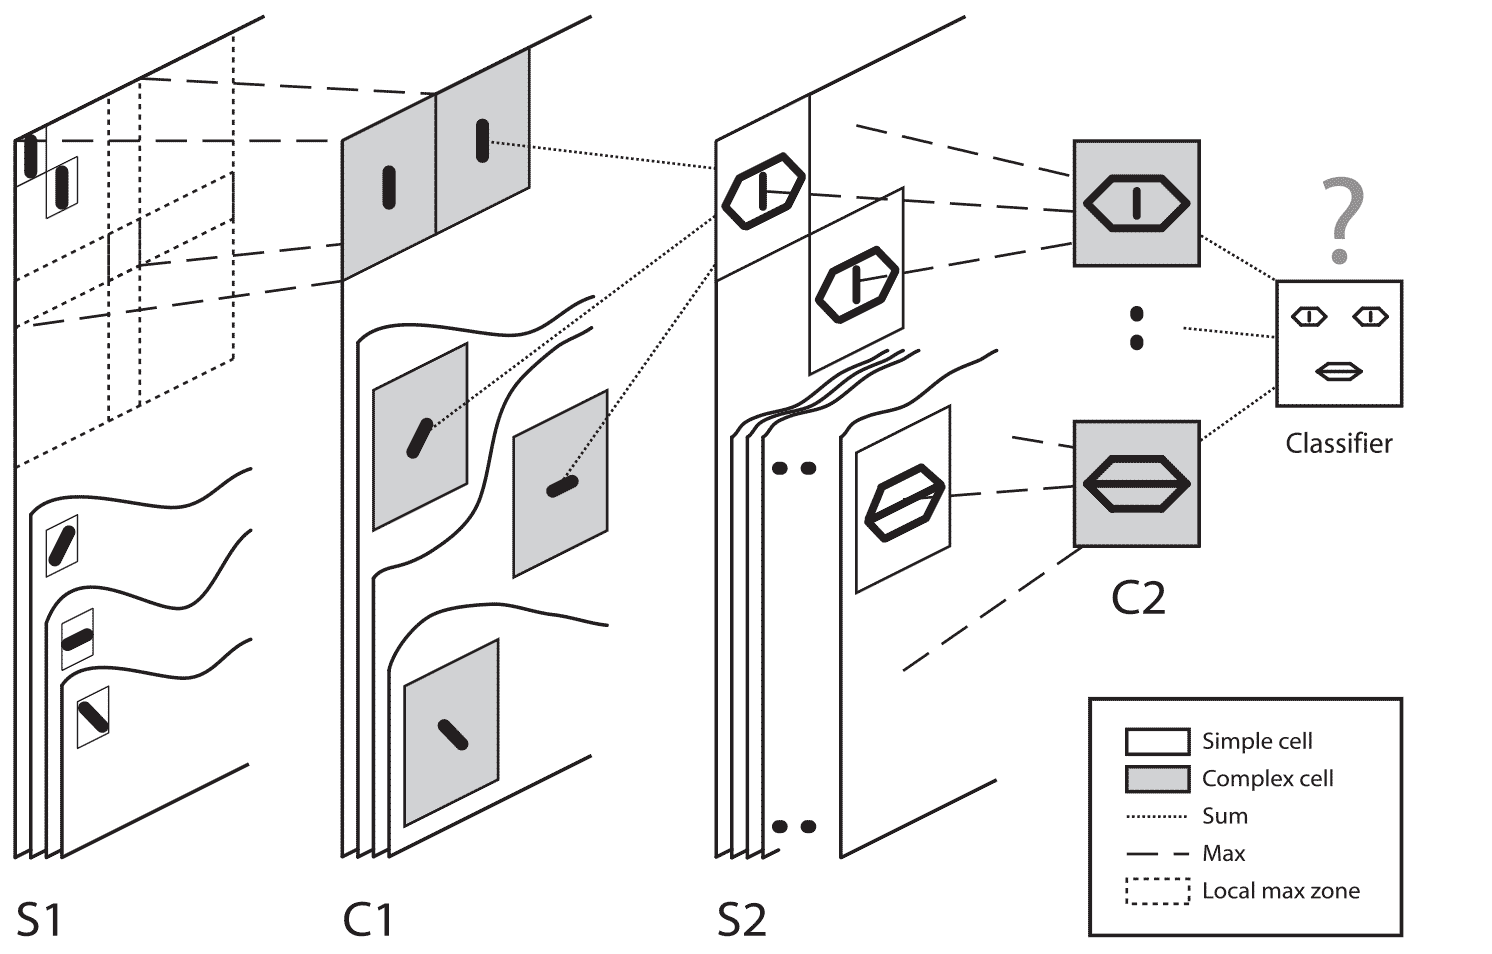
\includegraphics[height=9cm]{masquelier_model}
\caption[ساختار پیش‌خور مدل یادگیری ویژگی‌های بصری]{ساختار پیش‌خور مدل یادگیری ویژگی‌های بصری: مشابه \lr{HMAX}\cite{riesenhuber1999hierarchical} در این مدل نیز به صورت تناوبی سلول‌های ساده و سلول‌های پیچیده قرار داده شده است. سلول‌های \lr{S1} لبه‌ها را تشخیص می‌دهند. \lr{C1} نقشه‌های \lr{S1} را با بیشینه کردن پاسخ در یک همسایگی مربع از آن زیرنمونه می‌گیرد. \lr{S2} نسبت به ویژگی‌های پیچیده‌ی میانی گزیننده شده و ترکیبی از لبه‌های جهت‌دار را می‌دهند. سپس \lr{C2} بشینه‌ی پاسخ سلول‌های \lr{S2} در تمام موقعیت‌ها و مقیاس‌ها را منتقل می‌کند.\cite{masquelier2007unsupervised}}
\label{fig:masquelier_model}
}
\end{figure}

در هر گام، زمان اولین ضربه نسبت به آغاز محرک (مرتبه\footnote{\lr{Rank}} اولین ضربه) اصلی‌ترین متغیری هست که اطلاعات را در خورد جای داده و بر اساس ساختار مدل به نورون‌های پایین دست منتقل می‌شود. با نمایش یک محرک، سلول‌های \lr{S1} لایه‌ی اول، لبه‌ها را در چهار جهت اصلی (مشابه \lr{V1} در قشر بینایی) شناسایی می‌کند به این صورت که  هر چه قوی‌تر فعال شود، زودتر آتش خواهد کرد. تبدیل شدت-تاخیر\footnote{\lr{Intensity–latency conversion}} با سازوکاری که در ثبت‌های صورت گرفته از \lr{V1} مشاهده شده، که کاهش تاخیر را با کاهش کنتراست\cite{albrecht2002visual} و نزدیکی جهت محرک با جهت گزینندگی نشان می‌دهد\cite{celebrini1993dynamics}، منطبق است. تعداد ضربه‌ها در \lr{S1} از طریق مکانیسم رقابتی one-winner-take-all محدود شده و تنها ضربه متناظر با بهترین جهت در هر مکان منتقل می‌شود که در نتیجه تعداد ضربه‌ها را به یک چهارم کاهش می‌دهد. در چارچوب جاری، عملیات max متناظر است با انتشار اولین ضربه‌ی واصله از یک گروه آوران. چنین کاری را می‌توان با یک نورون تجمیع و آتش با حد آستانه‌ی پایین که اتصال از تمام گروه نورونی دارد انجام داد. 

فعالیت نورونی با محدود کردن یک ضربه به ازای هر نورون محدود شده است و در نتیجه تنها موج اولیه‌ی ضربه‌ها انتقال می‌یابد. از هر تصویر ورودی، چند مقیاس مختلف (پنج مقیاس در \cite{masquelier2007unsupervised}) پردازش می‌شود و به ازای هر مقیاس یک مسیر \lr{S1}-\lr{C1}-\lr{S2} وجود داشته و بنابراین اندازه‌ی میدان‌های تاثیر سلول‌های \lr{S2} متفاوت است. سپس سلول‌های \lr{C2} پاسخ بیشینه (اولین ضربه) را در میان سلول‌های \lr{S2} از میان همه‌ی موقعیت‌ها و مقیاس‌ها می‌گیرند که در نتیجه پاسخ‌ها نسبت به موقعیت و مقیاس ناوردا خواهند شد.

معادل سلول‌های \lr{S1} را در ناحیه‌ی \lr{V1} مغز و\lr{C1} را در نواحی \lr{V1}-\lr{V2} مغز می‌توان پیدا کرد. سلول‌های \lr{S2} شبیه سلول‌های \lr{V4}-\lr{PIT} و \lr{C2} مشابه \lr{AIT} است. در نهایت ماژول طبقه‌بند عملا وظایف \lr{PFC} را انجام می‌دهد. مشاهدات نشان می‌دهد که یادگیری وزن‌های اتصالات \lr{C1}-\lr{S2} به کمک \lr{STDP} منجر به ویژگی‌های بصری با پیچیدگی میانی می‌شود که مشابه آن در مغز نیز مشاهده شده است. نورون‌های لایه‌ی \lr{S2} میدان تاثیر محدودی دارند. به عبارت دیگر، سلول‌های \lr{S2}، ضربه‌ها را از یک میدان تاثیر به ابعاد $s \times s$ از یک نقشه‌ی \lr{C1} متناظر با یک مقیاس تجمیع می‌کنند. علاوه بر آن از مکانیسم اشتراک وزن برای سلول‌های \lr{S2} استفاده شده است. 

\section{ماشین حالت مایع}
شبکه‌های عصبی ضربه‌ای نقش قابل توجهی در فهم ما از ساز و کار مغز در علوم اعصاب داشته‌اند. با این حال تقریبا تمام مدل‌های ساخته شده از اتصالات یا پارامتر‌های تصادفی\footnote{\lr{Stochastic}} بهره می‌برند. دلیل آن این است که ساخت یک شبکه‌ی مدل که مدارات\footnote{\lr{Circuitry}} یکسان با مغز، و یا حتی یک کشت یاخته عصبی، داشته باشد غیر ممکن می‌نماید. در کشت یاخته، نورون‌ها قبل از تمایز سلولی\footnote{\lr{Cell Differentiation}}، ابتدا داخل ظروف پتری\footnote{\lr{Petri dishes}} قرار می‌گیرند تا رشد و داخل ظرف تشکیل شبکه دهند. اتصالات کشت‌های سلولی به صورت تصادفی ساخته می‌شوند. همچنین در مغز، در طول دوره‌ی رشد، «تصادفی بودن\footnote{\lr{Randomness}}» در تشکیل تعداد بالای اتصالات سیناپسی نقش دارد. مدعای واضح این امر این است که پیچیدگی نجومی ساختار مغز امکان ندارد که صرفا توسط ژنوم کد شده باشد؛ با این حال هر ارگانیسم مستقل، پس از یادگیری مناسب در محیط طبیعی و بهینه‌سازی توپولوژی و قدرت اتصالات سیناپسی، امکان فعالیت و بقا در محیط طبیعی را دارد. شبکه‌های عصبی مصنوعی نیز مانند مغز از این اصل پیروی می‌کنند: شبکه‌ی عصبی با اتصالات تصادفی ساخته شده و سپس با الگوریتم‌های یادگیری، وزن‌ها یا توپولوژی سیناپسی را اصلاح و بهینه می‌کند. به عبارت دیگر، تقریبا همه‌ی شبکه‌های عصبی، چه درون‌جاندازی\footnote{\lr{in vivo}}، چه درون‌کشتگاهی\footnote{\lr{in vitro}} یا درون‌رایانه‌ای\footnote{\lr{in silico}}، ذات تصادفی دارند. این امر علوم اعصاب را به سوالات بسیاری رهنمون می‌کند: با توجه به اینکه هدف غایی در علوم اعصاب فهم ساز و کار مغز است، چگونه با در بر داشتن این میزان بالا از عدم قطعیت و تصادفی بودن، مغز می‌تواند به طور عادی عمل کند؟ آیا این تصادفی بودن در نحوه‌ی عملکرد نقش مثبتی دارد یا به آن لطمه وارد می‌کند؟ یا به طور بنیادی‌تر، آیا یک شبکه‌ی عصبی تصادفی امکان پردازش اطلاعات زمانی‌فضایی\footnote{\lr{Spatiotemporal}} را بدون یادگیری دارد؟ و با در نظر گرفتن چنین حالتی، آیا مغز از این توانمندی شبکه‌های تصادفی منفعتی می‌برد؟ 

\subsection{پیش‌زمینه}
تقریبا تمام محرک‌های حسی به پاسخ‌های فضایی‌مکانی به فرم پتانسیل‌های عمل\footnote{\lr{Action Potentials}} منجر شده و به دستگاه عصبی مرکزی  منتقل می‌شوند. دنباله‌های سلسله‌ی پتانسیل‌های عمل را معمولا دنباله‌ی ضربه\footnote{\lr{Spike train}} می‌نامند که می‌توان آنها را فرایند‌های نقطه‌ای\footnote{\lr{Point processes}} دانست که در آن هر داده نمایانگر زمان وقوع یک پتانسیل عمل است. نورون‌ها از طریق پتانسیل‌های عمل ارتباط برقرار می‌کنند؛ با این حال شکل هر پتانسیل عمل در انتقال اطلاعات نقش چندانی ندارد و از این روی است که پردازش زمان دنباله‌ی ضربه از اهمیت فراوانی در دستگاه اعصاب برخوردار است. با این حال، اکثر فهم فعلی ما از مغز متوجه پردازش اطلاعات فضایی\footnote{\lr{Spatial}} می‌باشد و نحوه‌ی عملکرد مغز در مواجهه با الگوهای زمانی\footnote{\lr{Temporal}} یا الگوهای پیچیده‌ی زمانی‌فضایی هنوز درک نشده است.

در پردازش سیگنال، تبدیل فوریه\footnote{\lr{Fourier Transformation}} برای تبدیل سیگنال از فضای زمان به فضای فرکانس معرفی می‌شود. به طور مشابه، حلزون گوش در گوش میانی نیز سیگنال صوتی را با یک نگاشت فرکانسی-مکانی کد می‌کند و به این نحو، بخش‌های مختلف حلزون، به فرکانس‌های مختلف پاسخ می‌دهند. تجزیه‌ی سیگنال‌های زمانی به نمایش فضا-فرکانس در سامانه‌ی شنوایی اهمیت بسیاری دارد. اما مغز چگونه زمان را بیان کرده و سیگنال‌های زمانی‌فضایی را پردازش می‌کند؟ در شبکه‌های عصبی مصنوعی پیش‌خور\footnote{\lr{Feed-forward}} سنتی، یکی از راههای نمایش زمان که اغلب کاربرد دارد «فضاسازی زمان\footnote{\lr{Time Spatialization}}» است که به معنی اضافه کردن زمان به عنوان یک بعد اضافی در فضا می‌باشد. اما این به وضوح خلاف اتفاقی است که در مغز می‌افتد. یک چارچوب نظری که تحت عنوان «محاسبات وابسته به وضعیت\footnote{\lr{State-Dependent Computation}}» معرفی شده است\cite{buonomano2009state} این گونه تبیین می‌کند که زمان به طور ذاتی در شبکه‌های عصبی زیستی نهفته شده است و اطلاعات فضایی‌زمانی با تکامل خط سیرهای عصبی\footnote{\lr{Neural Trajectories}} کد می‌شود. این ایده مشابه مفهوم فضا-حالت در نظریه‌ی کنترل است که در آن هر نقطه در حالت-فضای سیستم، نمایانگر یک وضعیت سیستم بوده و یک خط سیرِ فضا-حالت نحوه‌ی تغییر سیستم در طول زمان در پاسخ به یک ورودی خارجی زمان-متغیر\footnote{\lr{Time-varying}} را نشان می‌دهد. وضعیت سیستم در هر نقطه از زمان نتیجه‌ی تاریخچه‌ی ورودی است. بنابراین، محرک‌های زمانی‌فضایی مختلف می‌توانند به خط سیرهای عصبی گوناگون بیانجامند. پس با مشاهده‌ی خط سیر‌ها، یا تغییر وضعیت شبکه در طول زمان، می‌توان به اطلاعاتی در مورد محرک ورودی، از جمله ماهیت آن، پی برد.

نظریه‌ی محاسبات وابسته به وضعیت، عموما تحت عنوان «محاسبات انباره‌ای\footnote{\lr{Reservoir Computing}}» شناخته شده و مبتنی بر شبکه‌های عصبی بازگشتی\footnote{\lr{Recurrent Neural Networks}} می‌باشد. ماشین حالت مایع\footnote{\lr{Liquid State Machine}} (\lr{LSM}) \cite{maass2002real} و شبکه‌ی انعکاس حالت\footnote{\lr{Echo State Network}} (\lr{ESN}) \cite{jaeger2001echo} دو رسته‌ی اصلی از خانواده‌ی محاسبات انباره‌ای هستند. این دو مدل با وجود شباهت‌های زیاد، تفاوت‌های بنیادین در پیاده‌سازی دارند. در حالی که شبکه‌ی انعکاس حالت از شبکه‌های بازگشتی آنالوگ ساخته شده و تحلیل‌های ریاضیاتی را به کار می‌برد، ماشین حالت مایع بر مبنای شبکه‌های عصبی ضربه‌ای بوده و تلاش بر انطباق زیستی ساختار شبکه و پارامتر‌هایش از خصوصیات آن است. با این حال کاربرد اصلی هر دوی اینها در پردازش الگوهای زمانی‌فضایی به صورت بلادرنگ\footnote{\lr{Real-time}} برشمرده می‌شود.

از منظر ماشین‌های کرنل، مشابه روش‌های کرنل در ماشین بردار پشتیبان\footnote{\lr{Support Vector Machine}} (\lr{SVM})، محاسبات انباره‌ای به یک رسانه‌ی برانگیختنی\footnote{\lr{Excitable}} به عنوان کرنل (یا در اینجا انباره) نیاز دارد تا به صورت غیرخطی ورودی را به فضای ویژگی با ابعاد بالا تبدیل کند. نتیجه‌ی این تبدیل، خط سیرهایی در فضای حالت با ابعاد بالا خواهد بود. نام گذاری این روش منشا جالبی دارد. فرض کنید یک سنگ، داخل یک استخر آب پرتاب شده است و شما تنها امواج تشکیل شده در سطح آب را مشاهده می‌کنید. ادعای مطرح شده این است که صرف این مشاهده می‌توان خصوصیات سنگ، مانند شکل یا سرعت ورود آن به آب، را محاسبه کرد. «ماشین حالت مایع» یا «محاسبات انباره‌ای» بخاطر این تمثیل نام‌گذاری شده‌اند. انباره به عنوان آب در نظر گرفته شده و محرک خارجی همانند سنگ است. انباره‌ی \lr{LSM} یک ریزمدار قشری\footnote{\lr{Cortical Microcircuit}} است که از نورون‌های ضربه‌ای به عنوان واحد‌های سازنده استفاده کرده و اتصالات سیناپسی آن اغلب از شکل‌پذیری کوتاه مدت\footnote{\lr{Short-term Plasticity}} استفاده می‌کنند. توان محاسباتی جهان شمول\footnote{\lr{Universal Computational Power}} \lr{LSM} نیز مورد مطالعه قرار گرفته است.

\subsection{معماری}
یک ماشین حالت مایع از سه بخش تشکیل شده است:
\begin{itemize}
\item 
یک لایه‌ی ورودی
\item
یک فیلتر مایع (انباره)
\item
یک یا چند نورون خطی و بدون حافظه تحت عنوان لایه‌ی قرائت\footnote{\lr{Readout Layer}}
\end{itemize}

(شکل از \lr{LSM} نمونه)

نورون‌های ورودی محرک‌ها را در قالب دنباله‌های ضربه دریافت کرده و جریان الکتریکی به ریزمدار قشری (فیلتر مایع) تزریق می‌کنند. این سیناپس‌های ورودی، محرک را نه به همه‌ی نورون‌ها، بلکه به تعداد منتخبی از آنها، انتشار می‌دهند. از جهت مدارها و توپولوژی اتصالات در انباره، الزامات خاصی تعیین نشده است و صرفا یک شبکه‌ی تصادفی کافی می‌باشد. این امر به ما اجازه می‌دهد که هم به صورت شبیه‌سازی‌های درون‌رایانه‌ای و هم به صورت درون کشتگاهی بتوانیم فیلتر مایع را پیاده‌سازی کنیم. در حالت درون‌رایانه‌ای، فیلتر مایع از صدها نورون ضربه‌ای تشکیل می‌شود که با هزاران اتصال سیناپسی به صورت تصادفی به هم متصل هستند. بخاطر محدودیت‌ها از نظر قدرت محاسباتی، اندازه‌ی فیلتر مایع نمی‌تواند به اندازه‌ی کشت‌های نورونی متشکل از چند صد هزار نورون و چند میلیون سیناپس باشند. از آنجایی که هر نورون، دینامیک غیرخطی و اتصالات سیناپسی خود را داشته و اتصالات بازگشتی بین نورون‌ها برقرار است، هر نورون پاسخ متفاوتی به ورودی خارجی نشان می‌دهد. بنابراین فیلتر مایع به عنوان یک تصویر غیرخطی از محرک ورودی در یک فضای ویژگی با ابعاد بالاتر عمل می‌کند. ابعاد فضای تصویر شده، تعداد نورون‌ها در فیلتر مایع خواهد بود. همچنین یک لایه‌ی قرائت، همه (یا بخشی از) پاسخ‌ها را دریافت کرده و می‌تواند به نحوی آموزش داده شود که یک ابرصفحه در فضای حالت برای جداسازی محرک‌ها رسم کند. روش‌های آموزش مختلفی می‌توان برای لایه‌ی قرائت به کار برد؛ از جمله آنالیز افتراقی خطی\footnote{\lr{Linear Discriminant Analysis}} (\lr{LDA})، ماشین بردار پشتیبانی (\lr{SVM}) یا حتی رگرسیون ساده‌ی خطی. از آنجایی که قرائت به صورت خطی و بدون حافظه است، همه‌ی پردازش غیرخطی و زمانی بر عهده‌ی انباره می‌باشد. بنابراین، عملکرد \lr{LSM} به دینامیک آن و حافظه‌ی محوشونده‌اش\footnote{\lr{Fading Memory}} در انباره بستگی دارد. تنها بخشی از \lr{LSM} که نیاز به آموزش دارد لایه‌ی قرائت است و فیلتر مایع از این مورد بی‌نیاز است. به همین جهت پیاده‌سازی کل \lr{LSM} حتی با کشت نورونی زنده امکان‌پذیر بوده و تلاش‌هایی هم در این راستا صورت گرفته است. با این حال هنوز اینکه آیا شبکه‌های عصبی زنده به عنوان انباره مناسبت هستند محل سوال و تحقیق است اما چیزی که می‌توان امروزه ادعا کرد این است که استفاده از ماشین حالت مایع به عنوان یک طبقه‌بند می‌تواند کاربردهای متعددی در مهندسی داشته باشد.

\subsection{شبکه‌های عصبی درون‌رایانه‌ای}
رشد سریع و اعجاب‌آور توان محاسباتی کامپیوتر‌ها به ما این امکان را داده است که بتوانیم به ارزیابی مدل‌های محاسباتی از شبکه‌های عصبی که منطبق بر زیست‌شناسی و فیزیولوژی هستند بپردازیم. در حال حاضر تعداد انگشت شماری پروژه روی شبکه‌های مصنوعی با ابعاد بالای چند میلیون نورون و با درجات متفاوتی از دقت شبیه‌سازی و انطباق زیستی وجود دارند \cite{eliasmith2012large,markram2006blue}. مزیت شبیه‌سازی‌های رایانه‌ای در مقایسه با آزمایش‌های زیستی روی کشت‌های سلولی، کنترل کامل روی همه‌ی ابعاد و امکان تنظیم و ثبت تمام پارامتر‌های شبکه است. این به ما اجازه می‌دهد که از سطح مولکولی به سطح شبکه و در نهایت به سطح رفتاری ارتباطاتی را ترسیم کنیم که ما را به سمت فهم بهتر از عملکرد مغز سوق دهد. شبیه‌سازی \lr{LSM} به ما امکان مطالعه‌ی چنین ارتباطاتی را می‌دهد: اثر دینامیک نورونی و سیناپسی روی رفتار شبکه و عملکرد ماشین حالت مایع، توانایی شبکه‌های تصادفی در پردازش الگوهای زمانی‌فضایی، اثر شکل‌پذیری در عملیات شبکه و...

طرح اولیه و صحت ماشین حالت اولیه از شبیه‌سازی رایانه‌ای بدست آمده است و چارچوب این مفهوم با هدف درک بهتری از عملکرد مغز ارائه شده است. ادعا شده است که امکان مدل‌سازی مخچه توسط ساختار \lr{LSM} وجود داشته\cite{yamazaki2007cerebellum} و از طرفی هیپوکمپوس\footnote{\lr{Hippocampus}} مشابه \lr{SVM} جداسازی الگوها را انجام می‌دهد\cite{baker2003there,bakker2008pattern}. همانطور که گفتیم \lr{SVM} اساسا شباهت‌های بسیاری با \lr{LSM} دارد و البته \lr{LSM} در قیاس با \lr{SVM} از نظر زیستی بیشتر قابل پذیرش است؛ زیرا سازوکار آن مبتنی بر پتانسیل‌های عمل بوده و کرنل با مدارات نورونی پیاده‌سازی می‌شود. 

در کاربرد‌های مهندسی، توان \lr{LSM} در انجام وظایف مختلف در زمان بلادرنگ، از جمله بازشناسی گفتار\cite{schrauwen2008compact}، بازشناسی کلمه\cite{verstraeten2005isolated} و رباتیک\cite{joshi2004movement} نشان داده شده و ادعا می‌شود عملکرد آن با سیستم‌های مدرن بازشناسی الگو قابل قیاس است. لازم به ذکر است که تلاش‌هایی نیز در جهت فائق آمدن بر محدودیت‌های محاسباتی شبیه‌سازی با کامپیوتر‌های عادی صورت گرفته و بعضی از مطالعات به سمت مدارات مجتمع دیجیتال برنامه‌پذیر\footnote{\lr{Field-Programmable Gate Array}} (FPGA) گرایش پیدا کرده‌اند. 

\subsection{شبکه‌های عصبی درون‌کشتگاهی}
ساخت شبکه‌های عصبی درون‌رایانه‌ای که تمام جنبه‌های شبکه‌های عصبی زیستی را در خود بگنجانند ممکن است امکان‌پذیر نباشد. علت آن این است که تکنولوژی ثبت سلولی حاضر، تنها اجازه‌ی اندازه‌گیری بخش کوچک و محدودی از دینامیک نورونی و سیناپسی را می‌دهد. با این حال عامل‌های ناشناخته‌ی فراوانی مانند دینامیک‌های مولکولی، ترجمه و رونویسی ژنی وجود دارد که می‌توانند در یادگیری و حافظه دخیل باشند. برای نمونه تقویت بلند مدت\footnote{\lr{Long-term potentiation}} و تضعیف بلند مدت\footnote{\lr{Long-term depression}} (LTP/LTD) در نتیجه‌ی فعال شدن گیرنده‌های \footnote{\lr{N-Methyl-D-aspartic}}NMDA یا تحکیم حافظه که بیان ژن‌ها در آن دخیل است از جمله‌ی این عوامل هستند. به عنوان مثال، در شبکه‌های زیستی، فاکتور‌های زیادی، مانند سیگنال‌های کلسیمی، در تشکیل حافظه نقش دارند. حافظه‌ی کوتاه مدت لازمه‌ی پردازش اطلاعات زمانی است. تقویت و تضعیف سیناپس‌ها، طنین\footnote{\lr{Reverberation}} سیگنال به موجب اتصالات بازگشتی و ثابت زمانی غشایی در یک نورون، منابع اصلی حافظه در شبکه‌های شبیه‌سازی شده‌ی درون‌رایانه‌ای هستند؛ با این حال فاکتور‌های دیگری مانند سیگنال‌های کلسیمی به طور عادی در تحقیقاتی که از شبیه‌سازی بهره می‌برند مطالعه نشده و در نظر گرفته نمی‌شود.

به علاوه‌ی اینها، قدرت محاسباتی فعلی برای مدل‌سازی در این سطح دقت و جزئیات کافی نیست. در مقایسه با شبکه‌های زیستی که پردازش ورودی به صورت موازی و بلادرنگ صورت می‌گیرد، شبیه‌سازی‌های کامپیوتری بخاطر محدودیت‌هایی که دارند به طرز غیر قابل قبولی کند هستند.

شبکه‌های درون‌کشتگاهی توانایی غلبه بر این مشکلات را دارند ولی قابلیت مشاهده و کنترل بسیار محدود روی این شبکه‌های نورونی عوامل بازدارنده‌ی مهمی هستند. دستگاه‌های \lr{MEA}\footnote{\lr{Multielectrode array}} به جهت ثبت سیگنال نورونی توسط یکسری الکترود کاربرد دارند. به طور عادی، یک ظرف \lr{MEA} شامل ۶۰ یا ۲۵۲ الکترود است که می‌توانند برای ثبت پتانسیل‌های عمل از نورون‌ها یا تحریک الکتریکی آنها استفاده شوند. البته با وجود اینکه تنها صدها نورون از میان میلیون‌ها نورون یک کشت سلولی قابل ثبت هستند، تلاش‌های موثری در استفاده از شبکه‌های درون‌کشتگاهی برای انجام عملیات‌های مختلف صورت گرفته است. 

\section{مسئله‌ی تشخیص اشیا}
عموم فعالیت‌های روزانه‌ی ما بستگی به تعیین ماهیت دقیق و سریع اشیا محیط اطرافمان دارد. شاید این موضوع که ما به آسانی توانایی تشخیص و بازشناسی اشیا را داریم باعث نادیده گرفتن عظمت و دشواری این کار شود. ما می‌توانیم اشیا را با وجود تغییرات متنوعی در ظاهرشان، از میان دهها هزار دسته\footnote{تعداد دسته‌های بصری، حدود ۳۰۰۰ عدد تخمین زده شده‌اند.\cite{biederman1987recognition} یعنی یک کودک ۶ ساله باید هر روز به طور متوسط حدود ۱۴ شی در روز یاد بگیرد. یا یک شی به ازای هر ساعت بیدار بودن.} شی‌ای که از پیش می‌شناسیم و تنها ظرف کسری از ثانیه شناسایی کنیم. فهم کامل ساز و کارهای مغزی دخیل در این توانایی خارق‌العاده پیشرفت عظیمی در علم اعصاب به حساب خواهد آمد.
مهمترین علت دشواری تشخیص اشیا از نظر محاسباتی این است که هر شی خاص، به دلیل تغییر در موقعیت، حالت و نورپردازی و نیز حضور اشیای دیگر در مجاورت آن می‌تواند مجموعه‌ای نامتناهی از تصاویر مختلف که امکان پدیدار شدن روی شبکیه چشم ما را دارند تشکیل دهد. به عبارت دیگر، با اینکه امکان دارد یک شی را بارها مشاهده کرده باشیم، اما هرگز دو تصاویر کاملا مشابه از آن شی در شبکیه چشم ما تشکیل نمی‌شود. مغز ما علاوه بر اینکه این هزاران ورودی تصویری را به عنوان یک شی شناسایی می‌کند، تصویر شی دیگری را که حتی ممکن است تا حدی با تصاویر شی اول همبستگی داشته باشد را به عنوان شی‌ای مجزا شناسایی می‌کند.
بنابراین تشخیص اشیا عبارت است از تمایز قائل شدن دقیق برای هر شی (تعیین هویت) و یا دسته‌ای از اشیا (طبقه‌بندی) در میان تمام اشیا دیگر. این تمایز باید نسبت به مجموعه‌ای از تغییرات روی تصویر شبکیه‌ای آن شی (تغییراتی روی موقعیت، ابعاد و روشنایی شی) ناوردا باشد. 

\subsection{فرآیند محاسباتی تشخیص اشیا}
جهت انجام یک عمل تشخیصی، یک نمایش نورونی از صحنه‌ی بینایی (الگوی فعالیت جمعیتی نورونی) استفاده می‌شود تا یک تصمیم‌گیری (برای مثال حضور یک شی در تصویر) صورت پذیرد. از نظر محاسباتی مغز می‌بایست یک تابع تصمیم را به کار گیرد تا فضای نمایش نورونی را به وجود یا عدم وجود شی نگاشت دهد.

\begin{figure}
\centering
{\footnotesize
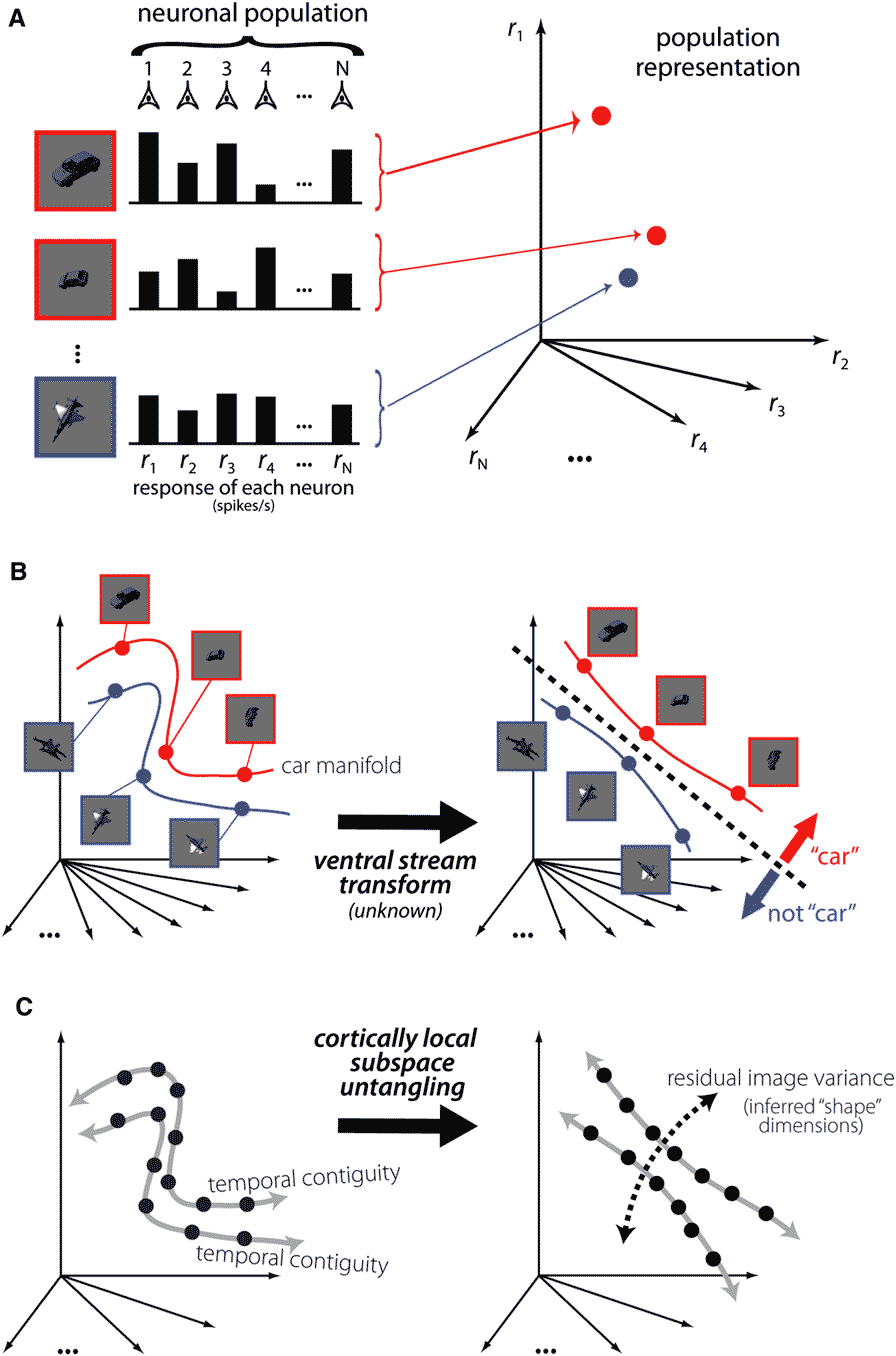
\includegraphics[height=17cm]{untangling}
\caption[از هم باز کردن نمایش شی]{از هم باز کردن نمایش شی: (A) الگوی پاسخ جمعیت نورون‌های بینایی (برای مثال سلول‌های گانگلیون) برای هر تصویر، نقطه‌ای در یک فضا با ابعاد بسیار است که در آن هر محور، سطح پاسخ هر نورون می‌باشد
(B) همه‌ی تبدیل‌های حافظ هویت از یک شی، یک خمینه با ابعاد پایین از نقاط را در فضای بردار جمعیت نمایش می‌دهند. جمعیت‌های نورونی در نواحی اولیه‌ی بینایی (سلول‌های گانگلیون، \lr{LGN} و \lr{V1}) شامل خمینه‌های هویت شی هستند که انحنای بسیاری داشته و در هم تنیده هستند (خمینه‌های قرمز و آبی) راه‌حل مسئله‌ی بازشناسی به نحو مفهومی، به صورت یکسری بازنمایش متوالی در طول مسیر شکمی (فلش مشکی) به یک نمایش جمعیتی جدید (\lr{IT}) تبیین می‌شود که امکان جداسازی و تمایز ساده بین خمینه‌های یک شی (خمینه قرمز برای خودرو) را با اشیای دیگر (خمینه آبی) را بدهد. از لحاظ هندسی این معادل آن است که به طوری نگاشت مجدد انجام شود که بتوان با یک جمع وزن‌دار ساده جداسازی صورت داد (یک اَبَرصفحه مانند خط مشکی منقطع) ت
(C) اکثر تصاویری که به صورت طبیعی تجربه می‌شوند برچسب (مانند «ماشین» یا «هواپیما») ندارند و مشابه شکل صرفا با یکسری نقاط در فضا مشخص شده‌اند. با این حال تصاویر با منشا یکسان (لبه یا شی) از لحاظ زمانی (فلش‌های طوسی) به هم نزدیک هستند. مشاهدات مبنی بر اهمیت این مجاورت برای \lr{IT} است.\cite{dicarlo2012does}}
\label{fig:untangling}
}
\end{figure}

اعمال این تابع تصمیم توسط نورون‌ها صورت می‌گیرد. درباره‌ی مکان و نحوه‌ی کد کردن و همچنین تعداد نورون‌هایی که در فرآیند تصمیم‌گیری وارد می‌شوند فرضیه‌های بسیاری مطرح است. اما مسئله‌ای که از نظر محاسباتی اهمیت بسزایی دارد این است که ساختار نمایش ورودی چه بوده و نوع توابع تصمیم‌گیری روی این نمایش چیست. یعنی می‌توان مسئله تشخیص اشیا را به صورت اعمال یک تابع غیرخطی پیچیده روی یک نمایش ابتدایی (مانند خروجی سلول‌های گانگلیون) در نظر گرفت یا در مقابل می‌توان عملگرهایی را یافت که این نمایش اولیه را مرحله به مرحله به نمایش‌های بهتری تبدیل کرده و برای یک تابع تصمیم‌گیرنده، به سادگی یک طبقه‌بند خطی، آماده کند.

واقعیت این است که از نظر محاسباتی تفاوتی بین این دو روش وجود ندارد اما روش دوم بیشتر به نحوه‌ی حل مسئله توسط مسیر شکمی دستگاه بینایی قرابت دارد. با توجه به اینکه استفاده از طبقه‌بندی غیرخطی و پیچیده از نظر عملکرد تغییر چندانی بوجود نمی‌آورد، استفاده از چنین رهیافتی (طبقه‌بندی خطی روی پاسخ جمعیتی نورون‌های \lr{IT}) کاملا موجه می‌نماید.

با توجه به آنچه گفته شد، می‌توان دلیل دشواری تشخیص اشیا از نظر محاسباتی را ساخت صور مناسب نمایش‌دهنده‌ی اشیا دانست. در یک دید جمعیتی از کد شدن اطلاعات، می‌توان هر تصویر را به صورت نقطه‌ای در فضایی با ابعاد برابر با جمعیت نورونی دانست. از این رو، مجموعه‌ی تمام نقاط نمایانگر تصاویر ممکن از یک شی در فضای نمایش سلولی یک مرحله، سطح پر پیچ و خمی را می‌سازند که به آن خمینه\footnote{\lr{Manifold}} گفته می‌شود. دستگاه بینایی بر مبنای یک ساختار سلسله مراتبی، به نحوی فضای نمایش را تغییر می‌دهد که خمینه‌های اشیای مختلف از درهم‌تنیدگی خارج گردند\cite{dicarlo2012does} (شکل \ref{fig:untangling}).

از آنجایی که تعداد مولفه‌های فضای نمایش نورونی با پیشروی در مسیر شکمی تغییر  می‌کند، می‌توان این تغییرات را نوعی مقیاس‌بندی چند بعدی در نظر گرفت که در نهایت منجر به صاف شدن\footnote{\lr{Flattening}} خمینه‌ی اشیا می‌شود. 

\section{مدل‌های ارائه شده برای مسیر اصلی دستگاه بینایی}
با در نظر گرفتن نحوه‌ی عملکرد سلول‌های عصبی، مشخصا در نواحی فراتر از \lr{V1}، مدل‌هایی برای عملکرد سلول‌های جریان شکمی ارائه شده است که می‌توان آنها را در سه دسته‌ی کلی که در ادامه می‌آید طبقه‌بندی کرد.

\subsection{مدل‌های عصب‌زیست‌شناختی}
بسیاری از مدل‌های حاضر جهت تشخیص اشیا بر پایه‌ی یافته‌های هوشمندانه‌ی هابل و ویزل از سلول‌های ساده و پیچیده‌ی قشر اصلی بینایی ارائه شده‌اند. 
هابل و ویزل با کشف سلول‌های ساده و پیچیده، بر اساس رفتار این سلول‌ها و با اطلاعاتی که از مسیر جریان اطلاعات بدست آوردند مدلی عصب‌زیست‌شناختی\footnote{Neurobiological} ارائه کردند. بر اساس این مدل، سلول‌های ساده به علت نوع خاص ورودی‌شان از سلول‌های \lr{LGN} که مراکز میدان تاثیرشان در راستای یک خط با جهت‌گیری مشخص است، این نوع پاسخ جهت‌گیری در یک راستا را تولید می‌کنند. 
در این مدل فرض بر آن است که سلول‌های پیچیده منحصرا تنها از سلول‌های ساده ورودی دریافت کرده و حاصل جمع خروجی‌های سلول‌های ساده با جهت ارجح یکسان ولی با میدان تاثیر متفاوت در یک همسایگی (موقعیت‌های مجاور یکدیگر) منجر به تولید میدان تاثیر سلول‌های پیچیده می‌شود. 

\subsection{مدل‌های الهام گرفته از مسیر بینایی}
مدل هابل و ویزل را می‌توان اینگونه خلاصه کرد که از سلسله مراتبی از سلول‌ها تشکیل می‌شود که در ابتدای آن، سلول‌هایی با تقارن مدور وجود دارند که همانند سلول‌های \lr{LGN} به نقاط کوچک نورانی قوی‌ترین پاسخ را می‌دهند. سپس سلول‌های ساده هستند که به نقاط نورانی پاسخ نمی‌دهند، بلکه به محرک‌های میله‌ای یا لبه‌ای در یک جهت و موقعیت خاص و با فاز معین پاسخ می‌دهند. در مرحله‌ی بعد سلول‌های پیچیده را داریم که آنها هم نسبت به میله‌های نورانی با یک جهت خاص گزینندگی دارند ولی نسبت به مکان و فاز محرک در میدان تاثیر‌شان حساس نیستند. در بالای این ساختار سلسله مراتبی سلول‌های فوق‌پیچیده\footnote{\lr{Hypercomplex cells} یا \lr{End-stopped cells}} نه تنها به مانند سلول‌های پیچیده به موقعیت و فاز میله‌های نورانی پاسخ ناوردا داشته، بلکه پاسخ آنها نسبت به طول میله‌ی نورانی نیز حساس است.

هابل و ویزل پیشنهاد دادند که چنین نمایش‌های به تدریج ناوردا و پیچیده‌ای می‌تواند از جمع ورودی‌های همگرا از سطوح پایین‌تر بدست آمده باشد. 

بسیاری از مدل‌های تشخیص اشیا از این ساختار سلسله‌مراتبی و همچنین ناوردایی و پیچیدگی فزاینده‌ی گزینندگی در طول آن، ایده گرفته‌اند. از اولین مدل‌هایی که چنین رویکردی را در پیش گرفت و ناوردایی به تغییرات مکان را در تصویر نشان می‌دهد، مدل Neocognitron بود. این مدل در سال ۱۹۸۰ توسط کانیهیکو فوکوشیما ارائه شد\cite{fukushima1980neocognitron} که البته از نسخه‌ی ابتدایی آن تا کنون تغییرات بسیاری در ساختار و قواعد حاکم بر آن مطرح شده است. 

\begin{figure}
\centering
{\footnotesize
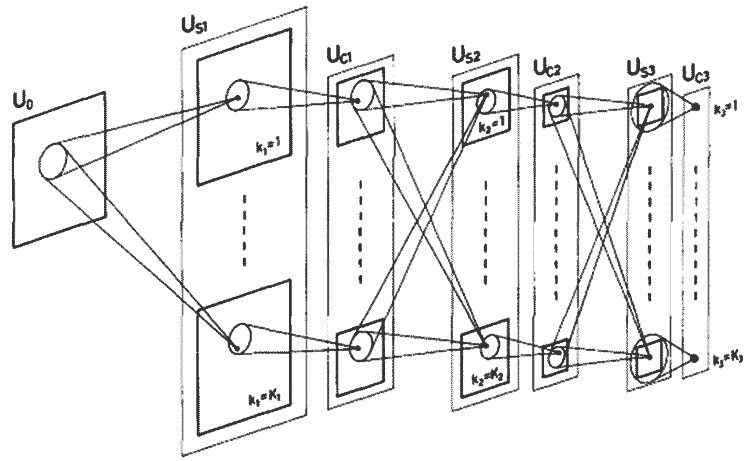
\includegraphics[height=8cm]{neocognitron}
\caption{ساختار لایه‌ای \lr{Neocognitron}\cite{fukushima1980neocognitron}}
\label{fig:neocognitron}
}
\end{figure}

این ساختار از یک لایه‌ی ورودی، متناظر با پیکسل‌های تصویر ورودی، تشکیل شده و بعد از آن به صورت یکی در میان، لایه‌های S و C (متناظر با سلول‌های ساده و پیچیده) قرار دارند. واحد‌های S ویژگی‌های مشخصی از ورودی را استخراج و با پیشروی در طول مسیر پیچیده‌تر می‌شود و واحد‌های C نیز منجر به ناوردایی به تغییرات مکانی خواهند شد (شکل \ref{fig:neocognitron}). 

\begin{figure}
\centering
{\footnotesize
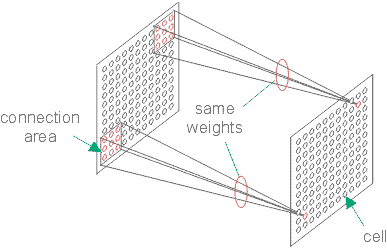
\includegraphics[height=6cm]{neocognitron2}
\caption{اشتراک وزنی}
\label{fig:neocognitron2}
}
\end{figure}

میدان تاثیر سلول‌های S نشان دهنده‌ی ویژگی‌های استخراج شده است و با هدف بهینه کردن عمل بازشناسی در طی فرآیند یادگیری صرفا اوزان اتصالات آوران به واحد‌های S میزان‌سازی می‌شود. در هر کدام از مراحل، دو لایه‌ی متوالی، به ترتیب از واحد‌های S و C قرار دارند و $U_{sl}$ نمایانگر لایه‌ای از سلول‌های S در مرحله‌ی $l$ام است. اتصالات ما بین دو لایه‌ی متوالی خاصیت رتینوتوپیک\footnote{\lr{Retinotopic}} دارند؛ به این معنی که مجاورت مکانی بین ویژگی‌ها را حفظ می‌کنند. همچنین در این مدل از قابلیت اشتراک وزنی\footnote{\lr{Weight sharing}} استفاده می‌شود و از این روی ضرایب اتصالات ورودی و اندازه‌ی میدان تاثیر سلول‌های یک لایه با یکدیگر برابر بوده ولی موقعیت‌های مختلفی را پوشش می‌دهند (شکل \ref{fig:neocognitron2}). 

مدل‌های متعدد دیگری با ایده گرفتن از ساختار سلسله مراتبی مسیر اصلی دستگاه بینایی توسعه یافته‌اند. مدل Neocognitron الهام‌بخش شبکه‌های عصبی پیچشی است که امروزه تحقیقات زیادی روی آنها متمرکز شده است. با وجود موفقیت نسبی این مدل‌ها در ماشین‌های تشخیص اشیا، هیچ کدام از آنها هنوز مدل کاملی برای مسیر اصلی بینایی ارائه نکرده‌اند.

\subsection{مدل‌های دارای انطباق زیستی}
مدل‌هایی که پیشتر معرفی شدند، اغلب بخاطر اینکه ایده اصلی‌شان را از ساختار زیستی مسیر بینایی الهام گرفته‌اند تا حدی قابل قبول‌اند؛ با این حال هیچکدام دارای سازوکارهای نورونی سازگار با یک سیستم زیستی نیستند. 
همانطور که بیان شد، ممکن است این نکته از نظرها پنهان بماند که دستگاه بینایی با چه چالش عظیمی در بازشناسی الگو از جمله تغییرات مکانی، زاویه‌ی دید و میزان روشنایی مواجه است. نقطه‌ی قوت دستگاه بینایی این است که با وجود دریافت محرک‌های متفاوت از یک شی، هنوز امکان تشخیص آن را دارد. پس دستگاه بینایی باید بتواند تغییرات در زاویه‌ی دید، موقعیت، اندازه و میزان نور را نادیده بگیرد. پس برای تعیین هویت اشیایی که از نظر فیزیکی مشابه‌اند باید بتوان آنها را تفکیک کرد ولی در مقابل برای طبقه‌بندی و دسته‌بندی اشیا باید بین اشیایی که از نظر فیزیکی متفاوتند تعمیم‌پذیری قائل شد.

به طور کلی برای شناخت، تعیین هویت و یا طبقه‌بندی یک شی باید نمایش بینایی آن با نمایشی که در حافظه قرار گرفته است مقایسه گردد. این چالش ما را به این سوال اساسی می‌رساند که اشیا چگونه در دستگاه بینایی نمایش داده می‌شوند.

دو دیدگاه مختلف از پس این پرسش برآمده است: دیدگاه اول بر این فرض استوار است که نتیجه‌ی تمام فعالیت‌های نورونی در مسیر اصلی بینایی، پدیدار کردن نمایشی است که در آن اشیا به صورت مجموعه‌ای از ویژگی‌های مشخص برای زاویه‌ی دید، نمایش یابند. به عبارت دیگر، در این دسته از مدل‌ها عمل تشخیص و بازشناسی به صورت تابعی از زوایای دید که از قبل تجربه شده‌اند می‌باشد. در مقابل آن، دیدگاه دوم که شامل مدل‌های توصیف ساختاری\footnote{\lr{Structural descriptions}} است را داریم. نظریه‌ی تشخیص با مولفه‌ها\footnote{\lr{Recognition-by-components}} (RBC) در سال ۱۹۸۷ توسط بیدرمن ارائه شده\cite{biederman1987recognition} و در آن فرآیند تشخیص شامل استخراج توصیفی ساختاری و ناوردا نسبت به زاویه‌ی دید از شی، بر حسب رابطه‌های فضایی میان مولفه‌های حجمی شی (تحت عنوان \lr{geon}) و سپس مقایسه آن با توصیف‌های ذخیره شده، می‌باشد. با این حال داده‌های بدست آمده از آزمایش‌های فیزیولوژی و روان‌فیزیکی\footnote{\lr{Psychophysical}} ناوردا بودن نمایش نهایی اشیا در مسیر بینایی نسبت به زاویه‌ی دید را رد کرده است و دیدگاه دوم از این منظر غیرقابل قبول است. ما نیز در ادامه دیدگاه اول را می‌پذیریم.